\RequirePackage[l2tabu, orthodox]{nag}
\documentclass{article}

\usepackage[letterpaper, margin=1.3cm]{geometry}
\usepackage{siunitx}
\usepackage{multicol}
\usepackage{pgfplots}
\usepackage{mathtools}
\usepackage{amssymb}
\usepackage{mathrsfs}
\usepackage{graphicx}
\usepackage{epstopdf}
\usepackage{float}
\usepackage{minted}
\usepackage{pdflscape}
\usepackage{subcaption}

\pgfplotsset{compat=1.16}

\title{ECE 302 Problem Set 1}
\author{Michael Kwok}
\begin{document}

\begin{titlepage}
     \begin{center}
          \vspace*{1cm}

          \textbf{Lab 1}

          \vspace{0.5cm}

          \Large{Introduction to Discrete-time Signals and Systems}
          \vspace{1.5cm}

          \textbf{Michael Kwok (1548454)}

          \vfill
          ECE 340 Lab Discrete Time Signals and Systems\\
          Department of Electrical and Computer Engineering\\
          University of Alberta\\
          30 September 2020
     \end{center}
\end{titlepage}
\begin{multicols*}{2}
     \section{Signal Generation and Plotting}
     2 signals were generated in this part of the lab, with the 2nd signal getting split into the real and imaginary part.
     \subsection{Signal plot}
     \begin{figure}[H]
          \centering
          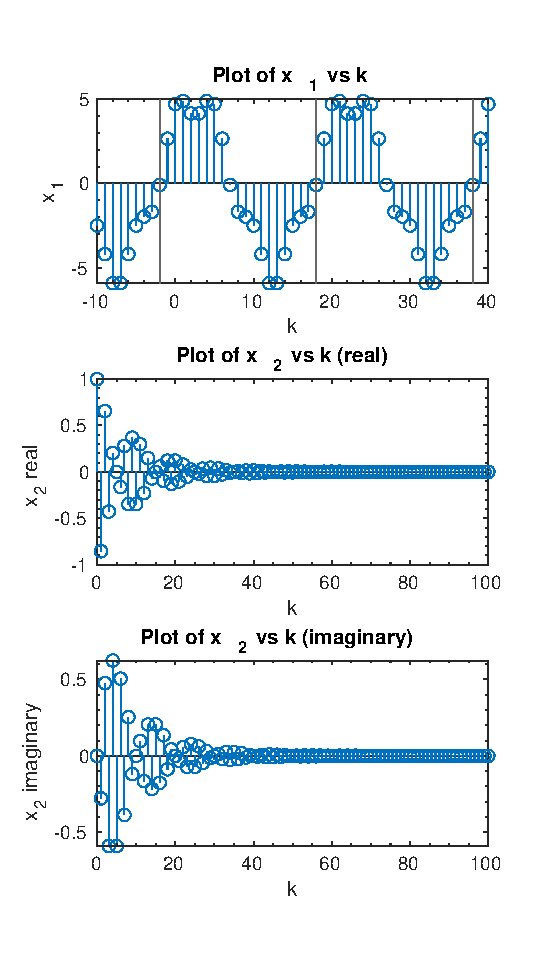
\includegraphics[width=\linewidth]{siggenres}
          \caption{Question 1a and b}
     \end{figure}
     \subsection{Periodicity of signals}
     In this lab, signal \(x_1\) is periodic while signal \(x_2\) is not periodic as \(x_1\) is linearly composed of two sinusoid signals while \(x_2\) is a damped sinusoid, which by definition is not periodic.

     Calculation of period:
     \begin{align*}
           & \omega_{\sin} = 0.1\pi, & f_{\sin} & = 0.05, & T_{\sin} = 20 \\
           & \omega_{\cos} = 0.4\pi, & f_{\cos} & = 0.2,  & T_{\cos} = 5
     \end{align*}
     Find LCM of  $T_{\sin}$ and  $T_{\cos}$ for base period
     \[LCM(T_{\sin}, T_{\cos})= 20\]
     Period of \(x_1\) is 20
     \subsection{Energy of signals}
     \begin{itemize}
          \item Energy of \(x_1\): \(698.5335\)
          \item Energy of \(x_2\): \(5.2632\)
     \end{itemize}

     \section{Audio Processing}
     \subsection{Song lyrics}
     Ho ey Ho ey baila baila comigo baila baila mi amor.
     \subsection{Audio signal}
     From the Matlab calculated result of 1000000 \(\times \) 1 which is a total of 1000000 samples in the audio file, which is almost 23 seconds \( \frac{1000000}{44100} \approx 22.68\). Screenshot of stem plot in appendix.
     \section{Image Processing}

     The image is 512 \(\times \) 512

     \begin{figure}[H]
          \centering
          \begin{subfigure}{0.4\linewidth}
               \centering
               
\includegraphics[width=\linewidth]{lena}
          \end{subfigure}
          \begin{subfigure}{0.4\linewidth}
               \centering
               
\includegraphics[width=\linewidth]{lena_bright}
          \end{subfigure}
          \caption{lena vs lena\_bright}
     \end{figure}

     \section{Audio Processing}
     \subsection{Difference equation}
     \(y(k) = a y(k-1) + x(k)\)
     \subsection{Calculation}
     \begin{enumerate}
          \item a = 0.5; \begin{align*}
                     y[0] & = 0 + 1                 \\
                          & = 1                     \\
                     y[1] & = 0.5 \cdot y[0] + x[1] \\
                          & = 1.5                   \\
                     y[2] & = 0.5 \cdot y[1] + x[2] \\
                          & = 1.75                  \\
                     y[3] & = 0.5 \cdot y[2] + x[3] \\
                          & = 1.875                 \\
                     y[4] & = 0.5 \cdot y[3] + x[4] \\
                          & = 1.9375                \\
                     y[5] & = 0.5 \cdot y[4] + x[5] \\
                          & = 1.96875
                \end{align*}
                \begin{figure}[H]
                     \centering
                     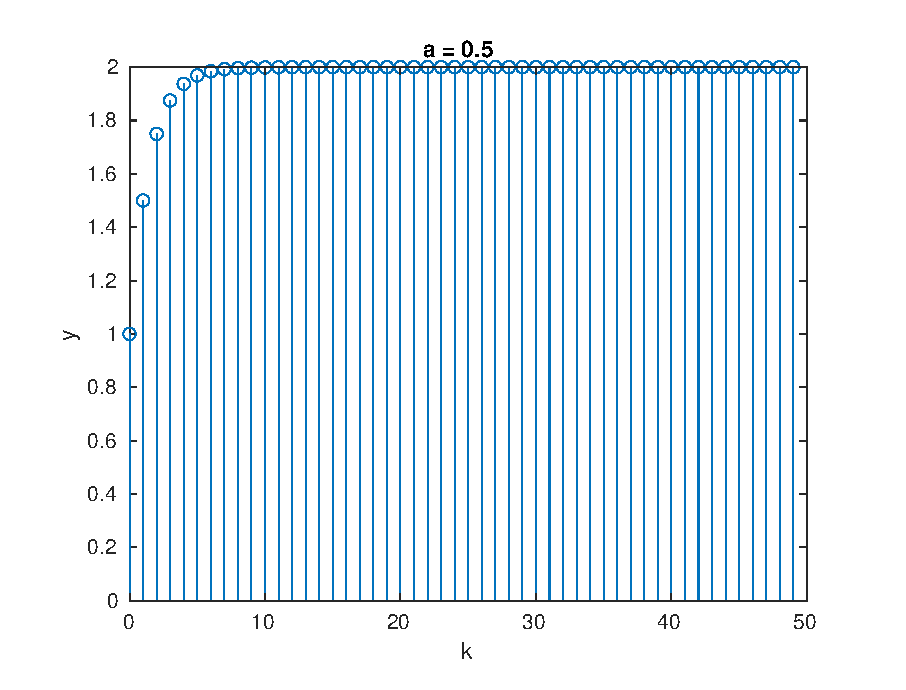
\includegraphics[width=\linewidth]{a5}
                     \caption{Graph at \(a=0.5\)}
                \end{figure}
          \item a = 2; \begin{align*}
                     y[0] & = 0 + 1               \\
                          & = 1                   \\
                     y[1] & = 2 \cdot y[0] + x[1] \\
                          & = 3                   \\
                     y[2] & = 2 \cdot y[1] + x[2] \\
                          & = 7                   \\
                     y[3] & = 2 \cdot y[2] + x[3] \\
                          & = 15                  \\
                     y[4] & = 2 \cdot y[3] + x[4] \\
                          & = 31                  \\
                     y[5] & = 2 \cdot y[4] + x[5] \\
                          & = 65
                \end{align*}
                \begin{figure}[H]
                     \centering
                     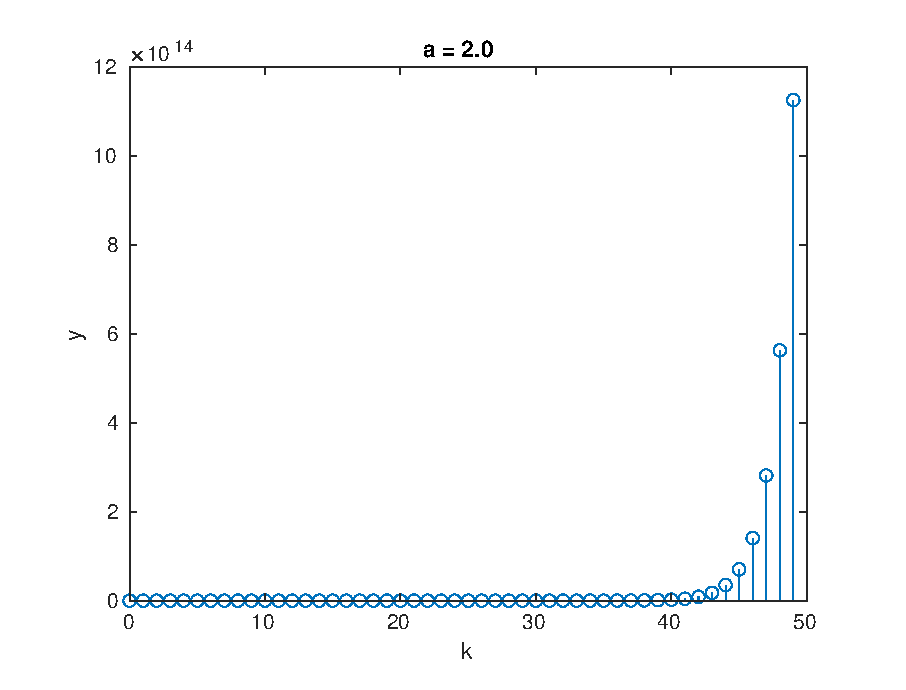
\includegraphics[width=\linewidth]{a2}
                     \caption{Graph at \(a=2\)}
                \end{figure}
          \item Another stable a = 0.1;
                \begin{figure}[H]
                     \centering
                     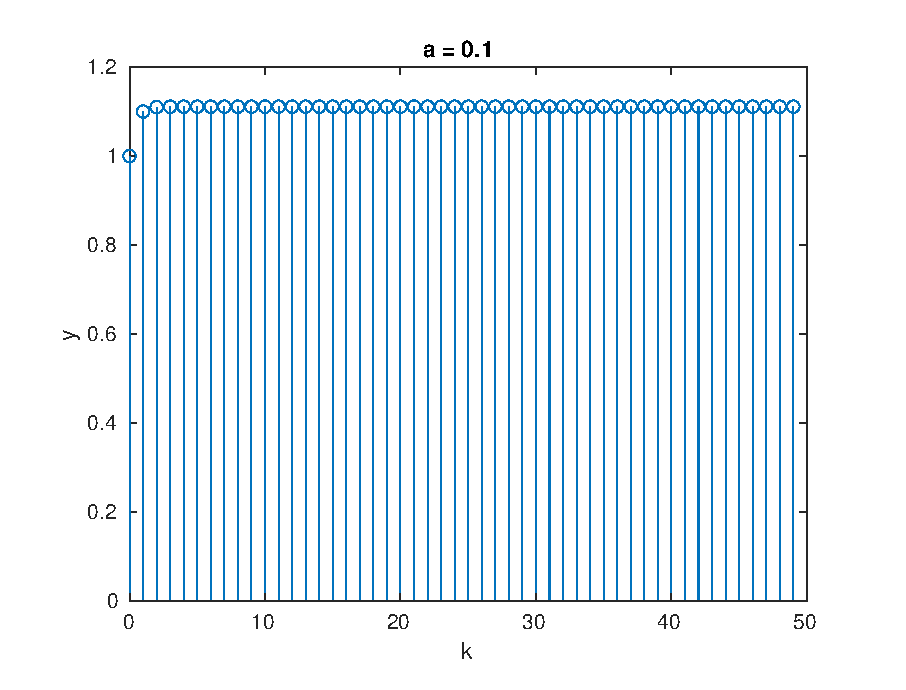
\includegraphics[width=\linewidth]{a1}
                     \caption{Graph at \(a=0.1\)}
                \end{figure}
     \end{enumerate}
     Any value \(|a| < 1\) will be stable. This is implied by the difference equation. A value \(|a| <1\) takes a fraction of the previous output before adding it to the current input. Eventually it reaches an unchanging value.

\end{multicols*}
\appendix
\begin{landscape}
     \section{Audio Plot}
     \begin{figure}[H]
          \centering
          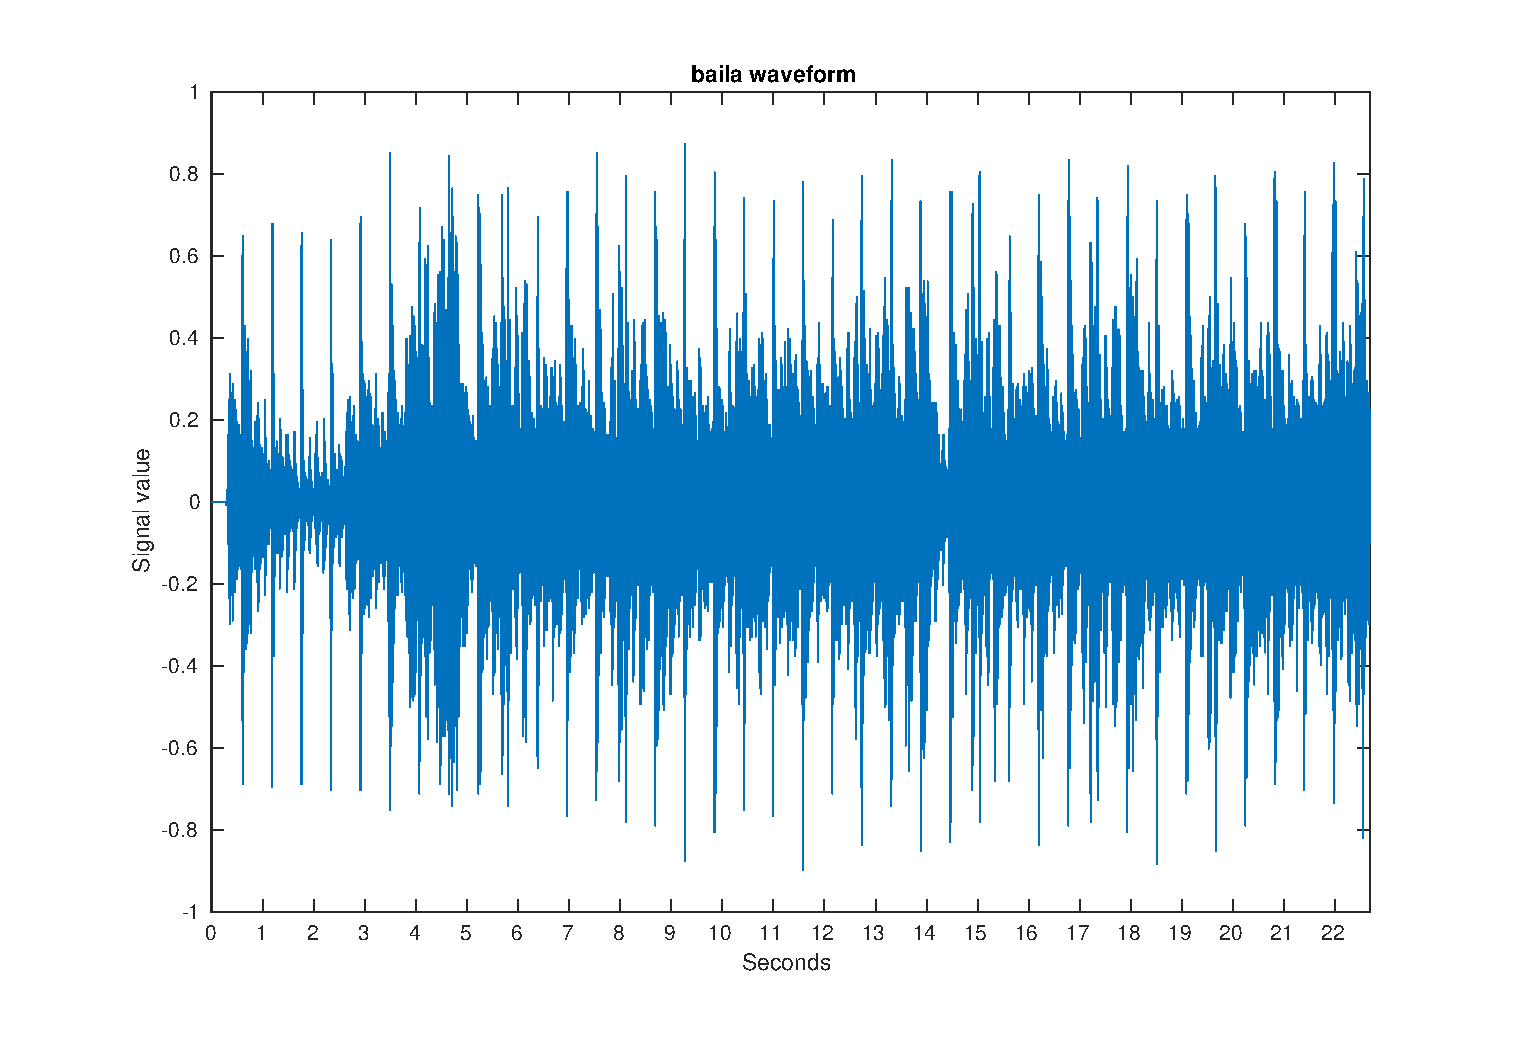
\includegraphics{baila}
          \caption{Audio plot}
     \end{figure}
\end{landscape}
\section{Main Code}
\inputminted{Matlab}{Lab1.m}
\section{sysresp Code}
\inputminted{Matlab}{sysresp.m}
\end{document}
